% -*- root: warwickthesis.tex -*-

\section{Introduction}
\label{sec:introduction-rep}

Another application of the STAMM model is the description of reprogramming of somatic cells to a pluripotent state as investigated in \cite{Armond:2013}. In the experimental setup a secondary mouse embryonic fibroblasts (MEFs) is used and transformed to a state of pluripotency \citep{Takahashi:2006hi,Jaenisch:2008cz}. More specifically we apply the model to genome-wide microarray gene expression time-course data obtained by \cite{SamavarchiTehrani:2010cp}. This transformation system has received a lot of attention and has been extensively studied in recent years; it has been suggested that the reprogramming process is inherently stochastic \citep{Hanna:2009ix}. Progress has also been made on single-cell investigations of the biological system \citep{Buganim:2012hp}. Questions still remain on genome-wide level, including the number of intermediate state between the initial MEF state and the final pluripotent state.

In this Chapter we start by briefly outlining results obtained by \cite{Armond:2013} when applying STAMM to a microarray data set in Section \ref{sec:iPsc-results}. Then (in Section \ref{sec:test-single-cell}) we discuss the main contribution in detail which is a comparative study of parameters obtained from STAMM and single-cell experiments performed by \cite{Buganim:2012hp}. The single-cell data was obtained by a new kind of experimental technique called a Fluidigm assay. This also illustrates an example of a possible next step in investigating a biological system once parameters from STAMM have been obtained. The main contributions to this work are:

\begin{itemize}
\item {\bf Computational} including verifying model selection results for both approaches (see below), comparison of multiple hyperparameters for Bayesian model selection and testing underlying structure of data.
\item {\bf Comparison} where estimated parameters from the model are compared to single-cell measurement.
\end{itemize}

\section{Results from STAMM}
\label{sec:iPsc-results}

\subsection{Differences in estimation}
\label{sec:diff-estim}

The initial step before we can make a comparison to single-cell results is to apply STAMM to the microarray time-course; obtaining single-cell level parameters and the number of states $K$. In  \cite{Armond:2013} there are differences in the estimation pipeline compared to the one outlined in Section \ref{sec:estim-pipe}, here we highlight the main differences.

The most important idea of a two-step estimation process is shared in both setups. The first difference is that the optimal number of clusters $\hat{m}$ is chosen by observing a plot of the k-means objective function; $\hat{m}$ is selected when an increase in the number of clusters does not significantly improve the objective function. The penalty for estimation used to regularise estimation in eqn. (\ref{eq:leastSqrs.indep}) is set to a small positive number (in this application set to $ \lambda = 0.1 $). Estimation of transition rates $\lbrace \mathbf{w} \rbrace $ is performed on genes closest to cluster centroids, instead of the cluster centroids themselves; then transition rates are fixed and estimation of expression signatures $\beta_{kj}$ is performed in the same way. Finally estimation of the number of states $\hat{K}$ is approached in two separate ways. The heuristic approach is to look at two quantities the model fit, i.e. the residual sum-of-squares (RSS), and the distinctness for individual state signatures quantified by the condition number $C = \max(s_i) / min(s_i)$; where $s_i$ are the singular values of a matrix made up of the expression signatures. To find the singular values of a matrix $A$ we need to compute the orthogonal matrices $U$ and $V$ and the matrix $D$ such that $A = V\, D \, U^T$, where $D$ is a diagonal matrix with its entries corresponding to the singular values. The other approach for finding an optimum number of states is employed for genes closest to centroids using ideas from Bayesian model selection. Let $\mathbf{y} = \lbrace y_j \rbrace$ denote observed data and $M_K$ the model with $K$ states. The posterior probability is $P(M_K | \mathbf{y}) \propto p(\mathbf{y}|M_K) $ with a flat prior distribution over models. The marginal likelihood $p(\mathbf{y} | M_K)$ accounts for the fit-to-data and model complexity. Writing all model parameters as $\theta = (\beta_{kj}, \lbrace \mathbf{w} \rbrace, \lbrace \sigma_j \rbrace) $ the marginal likelihood is:

\begin{equation}
  \label{eq:marginal-model}
  p(\mathbf{y} | M_K) = \int p(\mathbf{y} | \theta, M_K)\, p(\theta | M_K) d\theta.
\end{equation}

The marginal likelihood of the model eqn. (\ref{eq:marginal-model}) is computed using annealed importance sampling (AIS) \citep{Neal:2001ed}. Hyperparameters for this model are set by hand to reasonable values, see Supplement of \cite{Armond:2013} for details. The normalised score obtained for the marginal likelihood is the posterior probability for the number of states.

\subsection{Estimation results}
\label{sec:estimation-results}

The primary data used in \cite{Armond:2013} is obtained by reprogramming of a secondary mouse embryonic fibroblast (MEF) where Oct4, Sox2, Klf4, and cMyc are expressed under induction in the system for 30 days \citep{SamavarchiTehrani:2010cp}. Microarray measurements were made at $t = \lbrace 0, 2, 5, 8, 11, 16, 21, 30 \rbrace$ days after induction of expression factors. The microarray data is standardised per gene such that $y_j(t) = \left(z_j(t) - \mu_j \right) / \sigma_j$, where $z_j(t)$ is original $\log_2$ transformed data, $\mu_j$ is the mean and $\sigma_j$ is the standard deviation of the time course data for gene $j$. A total of $4383$ genes are retained out of the whole gene list after filtering out genes with small mean and standard deviation in their expression over time, as a way of removing uninformative genes. First genes in the bottom quartile of the mean and from the remaining set we remove genes in the bottom quartile of standard deviation.

\begin{figure}[!t]
  \centering
  % 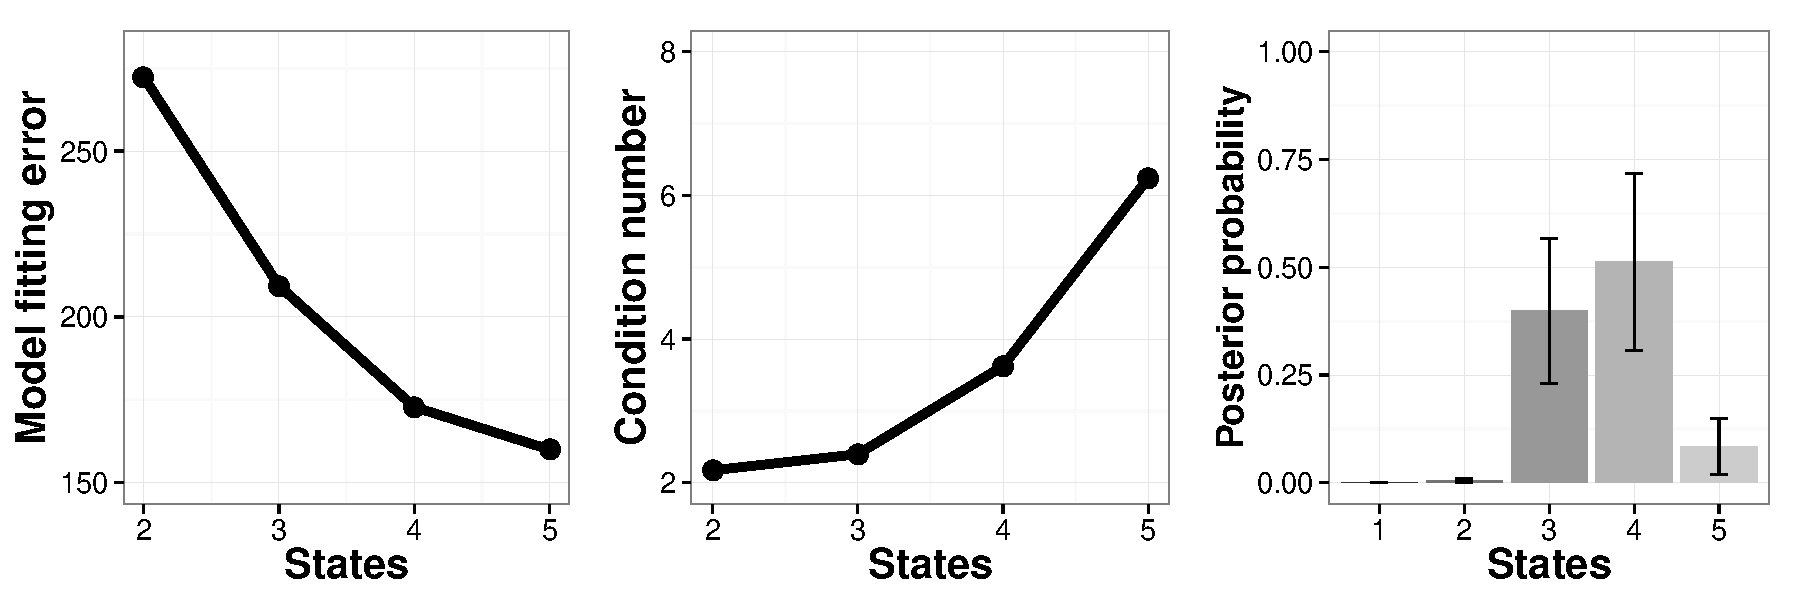
\includegraphics[width=1\textwidth]{pics/rss_rcond_bay1.pdf}
  \subfigure[RSS]{
    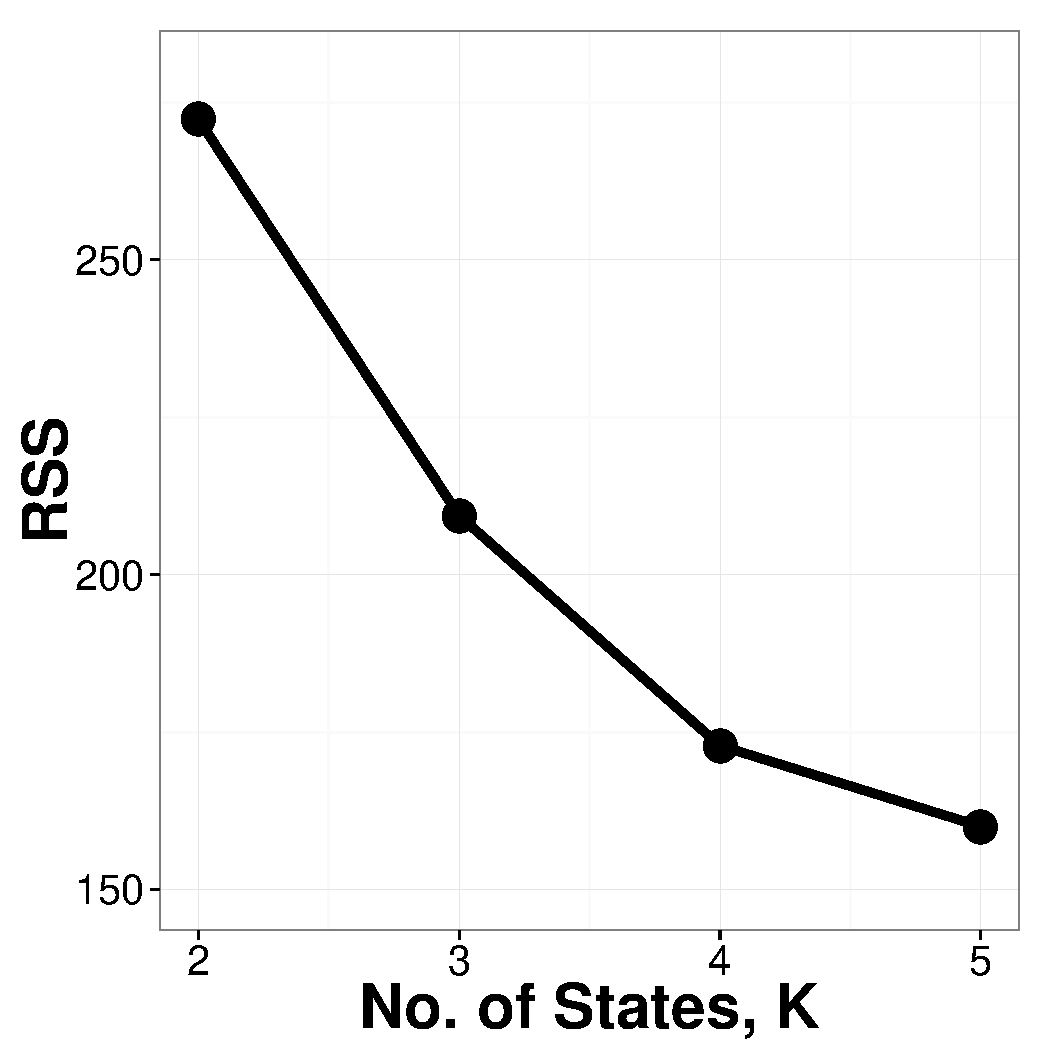
\includegraphics[width=0.3\textwidth]{pics/rss.pdf}
  }
  \subfigure[Condition number]{
    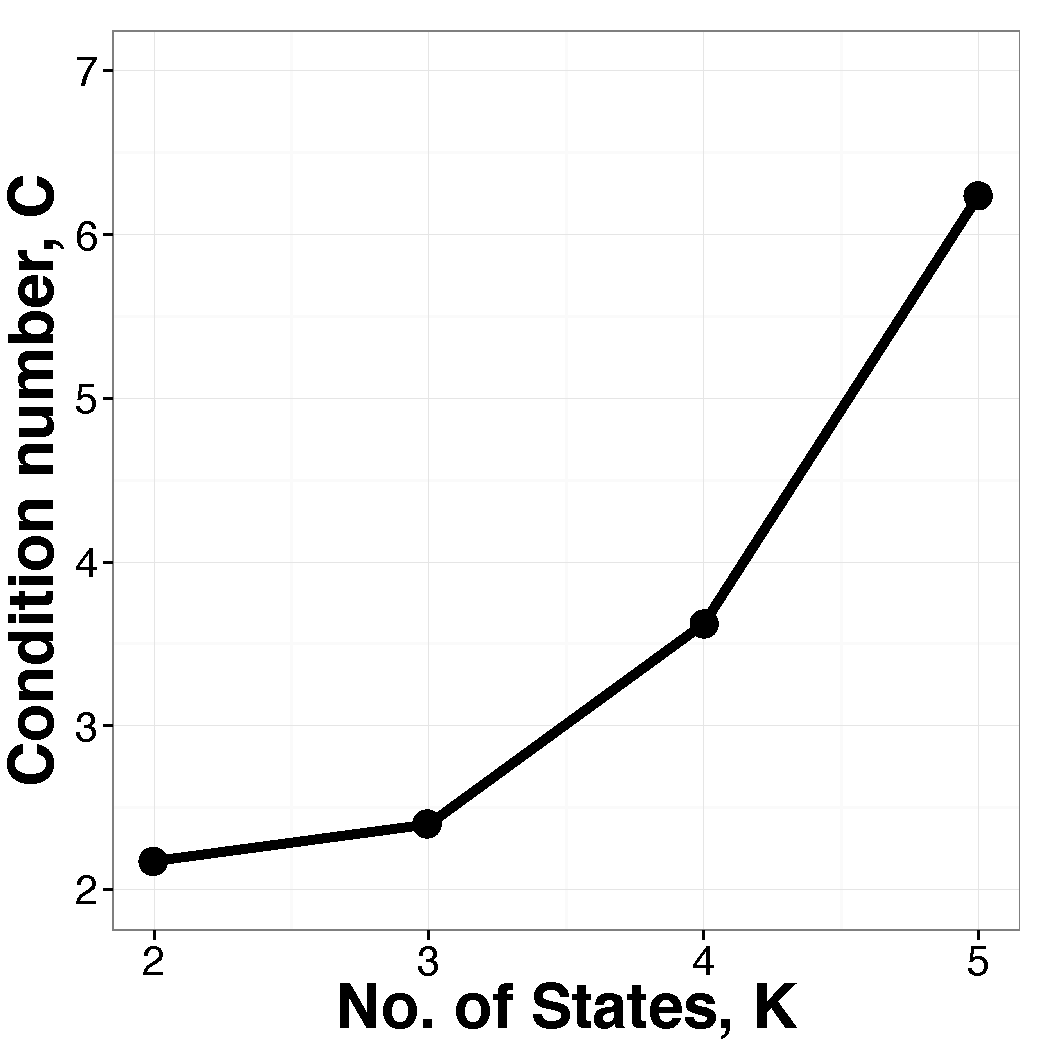
\includegraphics[width=0.3\textwidth]{pics/rcond.pdf}
  }
  \subfigure[Posterior probability]{
    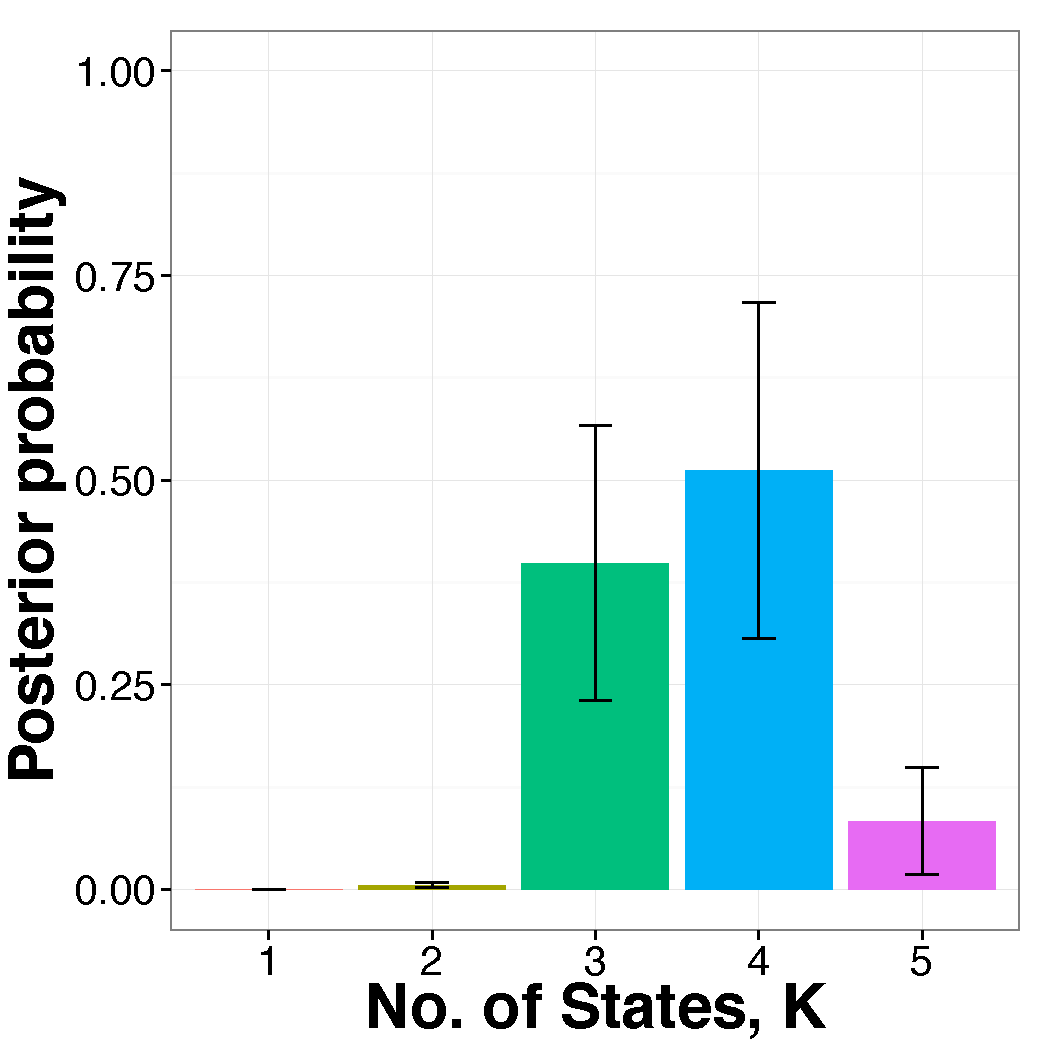
\includegraphics[width=0.3\textwidth]{pics/rep_bayes.pdf}
  }
  \caption{Application of STAMM to a microarray time-course (a) Plot of the model fit residual sum of squares (RSS). (b) Plot of the condition number for estimated expression signatures quantifying linear dependence between states. A larger number corresponds to more dependence. (c) Posterior probabilities obtained from Bayesian model selection (see Section \ref{sec:diff-estim} for details).}
  \label{fig:model-fit-repro}
\end{figure}

The number of clusters chosen for this data set of $8$ time points is $\hat{m} = 7$. As mentioned above, the penalty used in this application is $\lambda = 0.1$. With these parameters set, the transition rates are estimated from cluster representative genes. Once transition rates are fixed, the expression signatures for the remaining genes are estimated. The analysis is carried out for $K = \lbrace 2, \ldots, 5 \rbrace $ and results for model selection are summarised in Figure \ref{fig:model-fit-repro}. Unsurprisingly the RSS keeps decreasing for increasing $K$ (Figure \ref{fig:repro-rss}) since numbers of model parameters increase. To determine number of states heuristically, we compare these results with the condition number (Figure \ref{fig:repro-cond}). We find that the difference in condition number from $K=4$ to $K=5$ is larger than the preceding changes. This suggests that decrease in RSS from $4$ to $5$ states is mostly due to overfitting and the additional state is not distinct. The posterior probabilities form Bayesian model selection for $7$  genes closest to the centroid (see above for details), are shown in Figure \ref{fig:repro-bay}. Combined, these results indicate that a $\hat{K} = 4$ since it strikes a good balance between model fit and distinct expression signatures for states as well as having the highest posterior probability.

\begin{figure}
  \centering
  \subfigure[RSS]{
    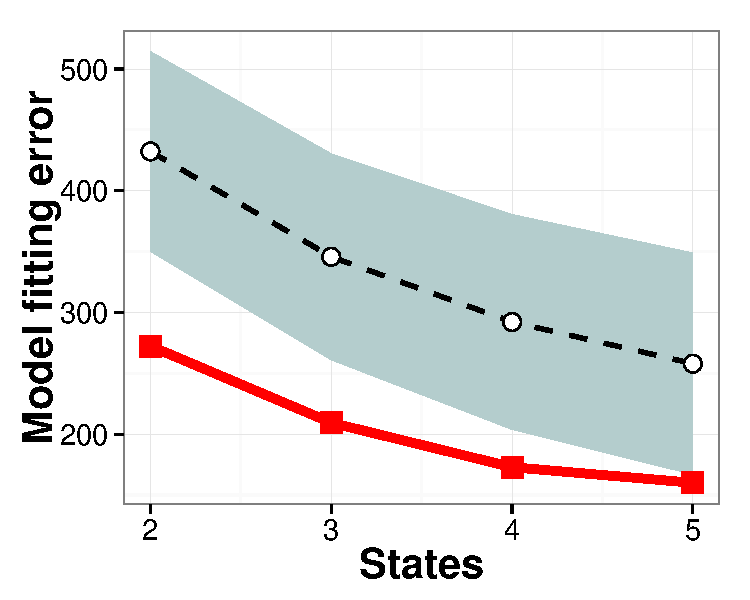
\includegraphics[width=0.3\textwidth]{pics/supp_fig_randomised3.pdf}
    \label{fig:repro-rss}
  }
  \subfigure[Condition number]{
    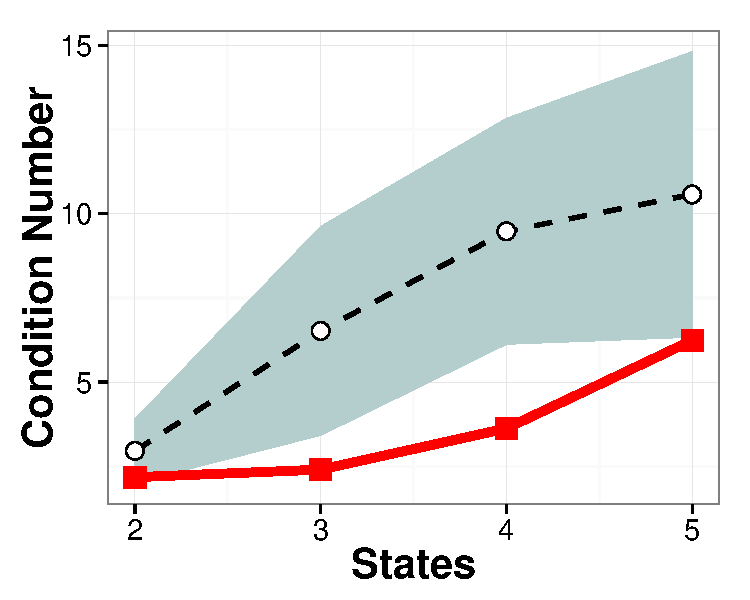
\includegraphics[width=0.3\textwidth]{pics/supp_fig_randomised4.pdf}
    \label{fig:repro-cond}
  }
  \subfigure[Bayesian model selection]{
    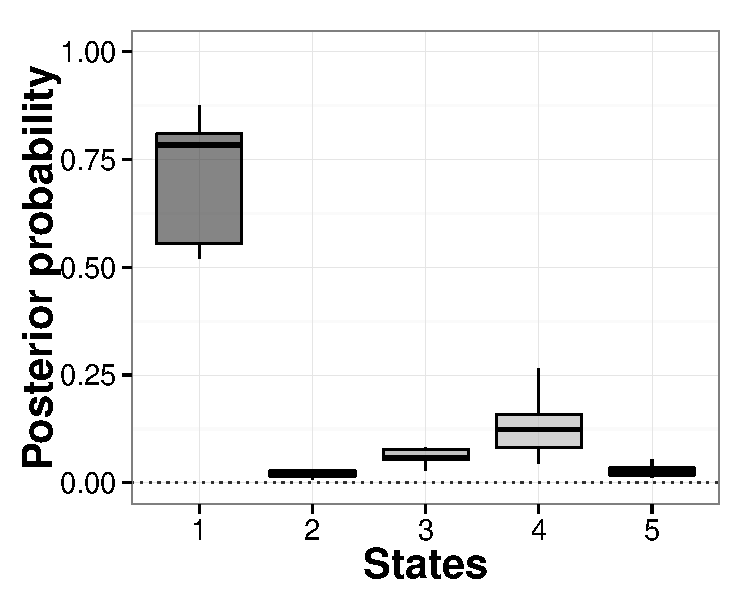
\includegraphics[width=0.3\textwidth]{pics/supp_fig_randomised1.pdf}
    \label{fig:repro-bay}
  }
  \caption{Random permutation of time points. The time points of data are randomly permuted ten times and parameter estimation is carried out for each case. \subref{fig:repro-rss} shows the RSS as a function of the number of states. \subref{fig:repro-cond} shows the condition number a measure for the independence of state-specific expression signatures. In \subref{fig:repro-rss} and \subref{fig:repro-cond} the solid red line show parameters for the original data and the dashed line represents the average of ten estimates and the dashed area represents a standard deviation. \subref{fig:repro-bay} shows posterior probabilities as a function of number of states calculated using Bayesian methods, results from ten estimations are summarised as box plots. For both RSS and condition numbers randomised data performs worse for all states. Bayesian model selection for the permuted data shows no indication that there are intermediate states. The data-set we use is obtained from \citep{SamavarchiTehrani:2010cp}.}
\label{fig:permutation-repro}
\end{figure}

\section{Testing against single-cell data}
\label{sec:test-single-cell}

\subsection{Single-cell experiment}
\label{sec:single-cell-exper}

Results in Section \ref{sec:estimation-results} are obtained analysing homogenate time-course data; but the transformation process itself takes place on a single-cell level therefore obtaining data single-cell level and studying the behaviour is tremendously valuable. Comparing results from STAMM to single-cell observations also indicates how well the underlying single-cell process is modelled. For this purpose we investigate the mRNA single-cell expression performed by \cite{Buganim:2012hp}. They also investigate a secondary MEF system reprogrammed by transduction of Oct4, Sox2, Klf4, and cMyc; obtaining data with the Fluidigm assay, resulting in $96$ single-cell measurements with gene expression from $48$ genes. Observations are made in populations, starting with MEFs, over cells at $2 - 6$ days during reprogramming, to the final reprogrammed cells.

\subsection{Comparing results}
\label{sec:comparing-results}

The single-cell measurements \citep{Buganim:2012hp} allow for analysis that has not been possible for population average data. Although important questions about the transformation process such as the number of states and transition rates still remain difficult to track down; due to the fact that each time a single-cell measurement is made the cell has to be destroyed and additional work is necessary to determine distinctive markers for known states for purification.

Given available data we can address interesting questions on expression patterns; since we assume that cells belonging to the same states would have a comparable expression patterns across observed genes. This is especially the case since measured genes are deemed important for reprogramming. To this end we cluster the data for all cells in a $48$ dimensional gene expression space. To perform the clustering we use a widely available clustering tool in R \texttt{mclust}; it employs a variety of multi-variate clustering methods and scores them using the Bayesian Information Criterion (BIC). The best performing method is shown in Figure \ref{fig:buganim-mclust}. We find that optimal number of clusters is $3$ since the BIC score starts decreasing for larger cluster sizes. \cite{Buganim:2012hp} suggest four clusters which they obtain using principle component analysis, which depends heavily on initial normalisation between samples.

\begin{figure}[!t]
  \centering
  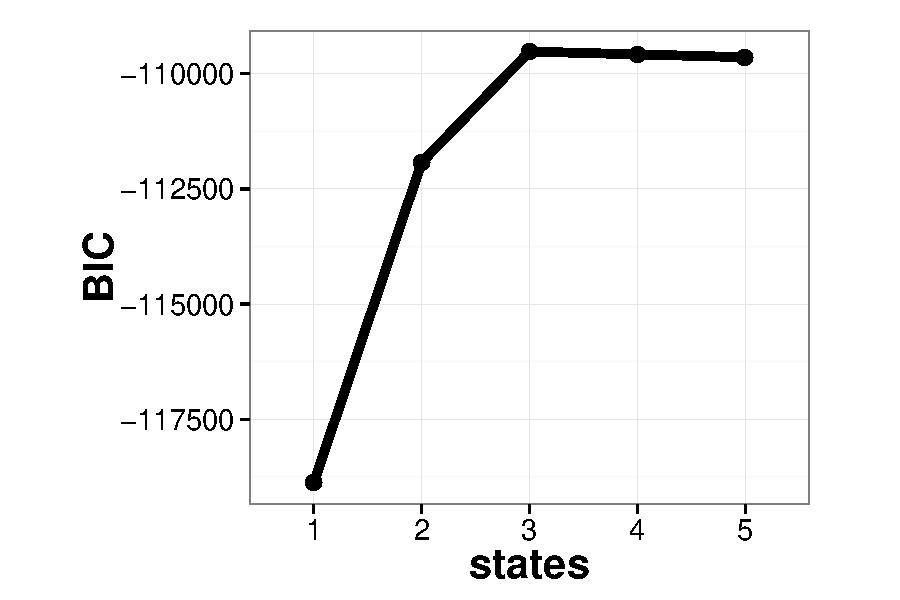
\includegraphics[width=0.6\textwidth]{pics/yossi_mclust.pdf}
  \caption{Single-cell expression levels in different experimental settings from \cite{Buganim:2012hp} are clustering using a standard clustering procedure in R called mclust. We use the Baysian Information Criterion (BIC) to score different cluster sizes. We find the optimal number of clusters to be $3$ since the BIC score decreases for larger cluster sizes.}
  \label{fig:buganim-mclust}
\end{figure}

Next, we try to determine if state specific expression signatures, estimated from microarray data, can be compared with this new single-cell data. Disregarding conditions for each cells measurement we assign each of the single-cell measurements to each of the states in the $K=4$ model. Since measurements are performed on different systems as well as a using different procedures we scale pre-processed data to be in the interval $[0, 1]$ by dividing the expression for a gene by its maximum expression over time. Then we compute the euclidean distance between gene expression on a single-cell level and estimated gene expression signatures and assign each cell to a specific state. The heatmap in Figure \ref{fig:buganim-heat} shows fractions of cells that are assigned to each state. All MEF conditions have a peak at $K=1$. Measurements obtained between $t=2$ and $t=44$ days are spread over state $K=1$ and $K=3$ with very few cells also in the second state. We do not find any cells, which have measurements close to the final state. Measurements for dox-independent and iPS cells occupy only the final two states. These results clearly show a transformation starting with MEF state and undergoing changes across intermediate states before reaching the final reprogrammed state. Of course, this is a very small study and studies made on a slightly different system under different conditions, therefore even the approximate similarities we find to our estimated parameters are promising.

\begin{figure}
  \centering
  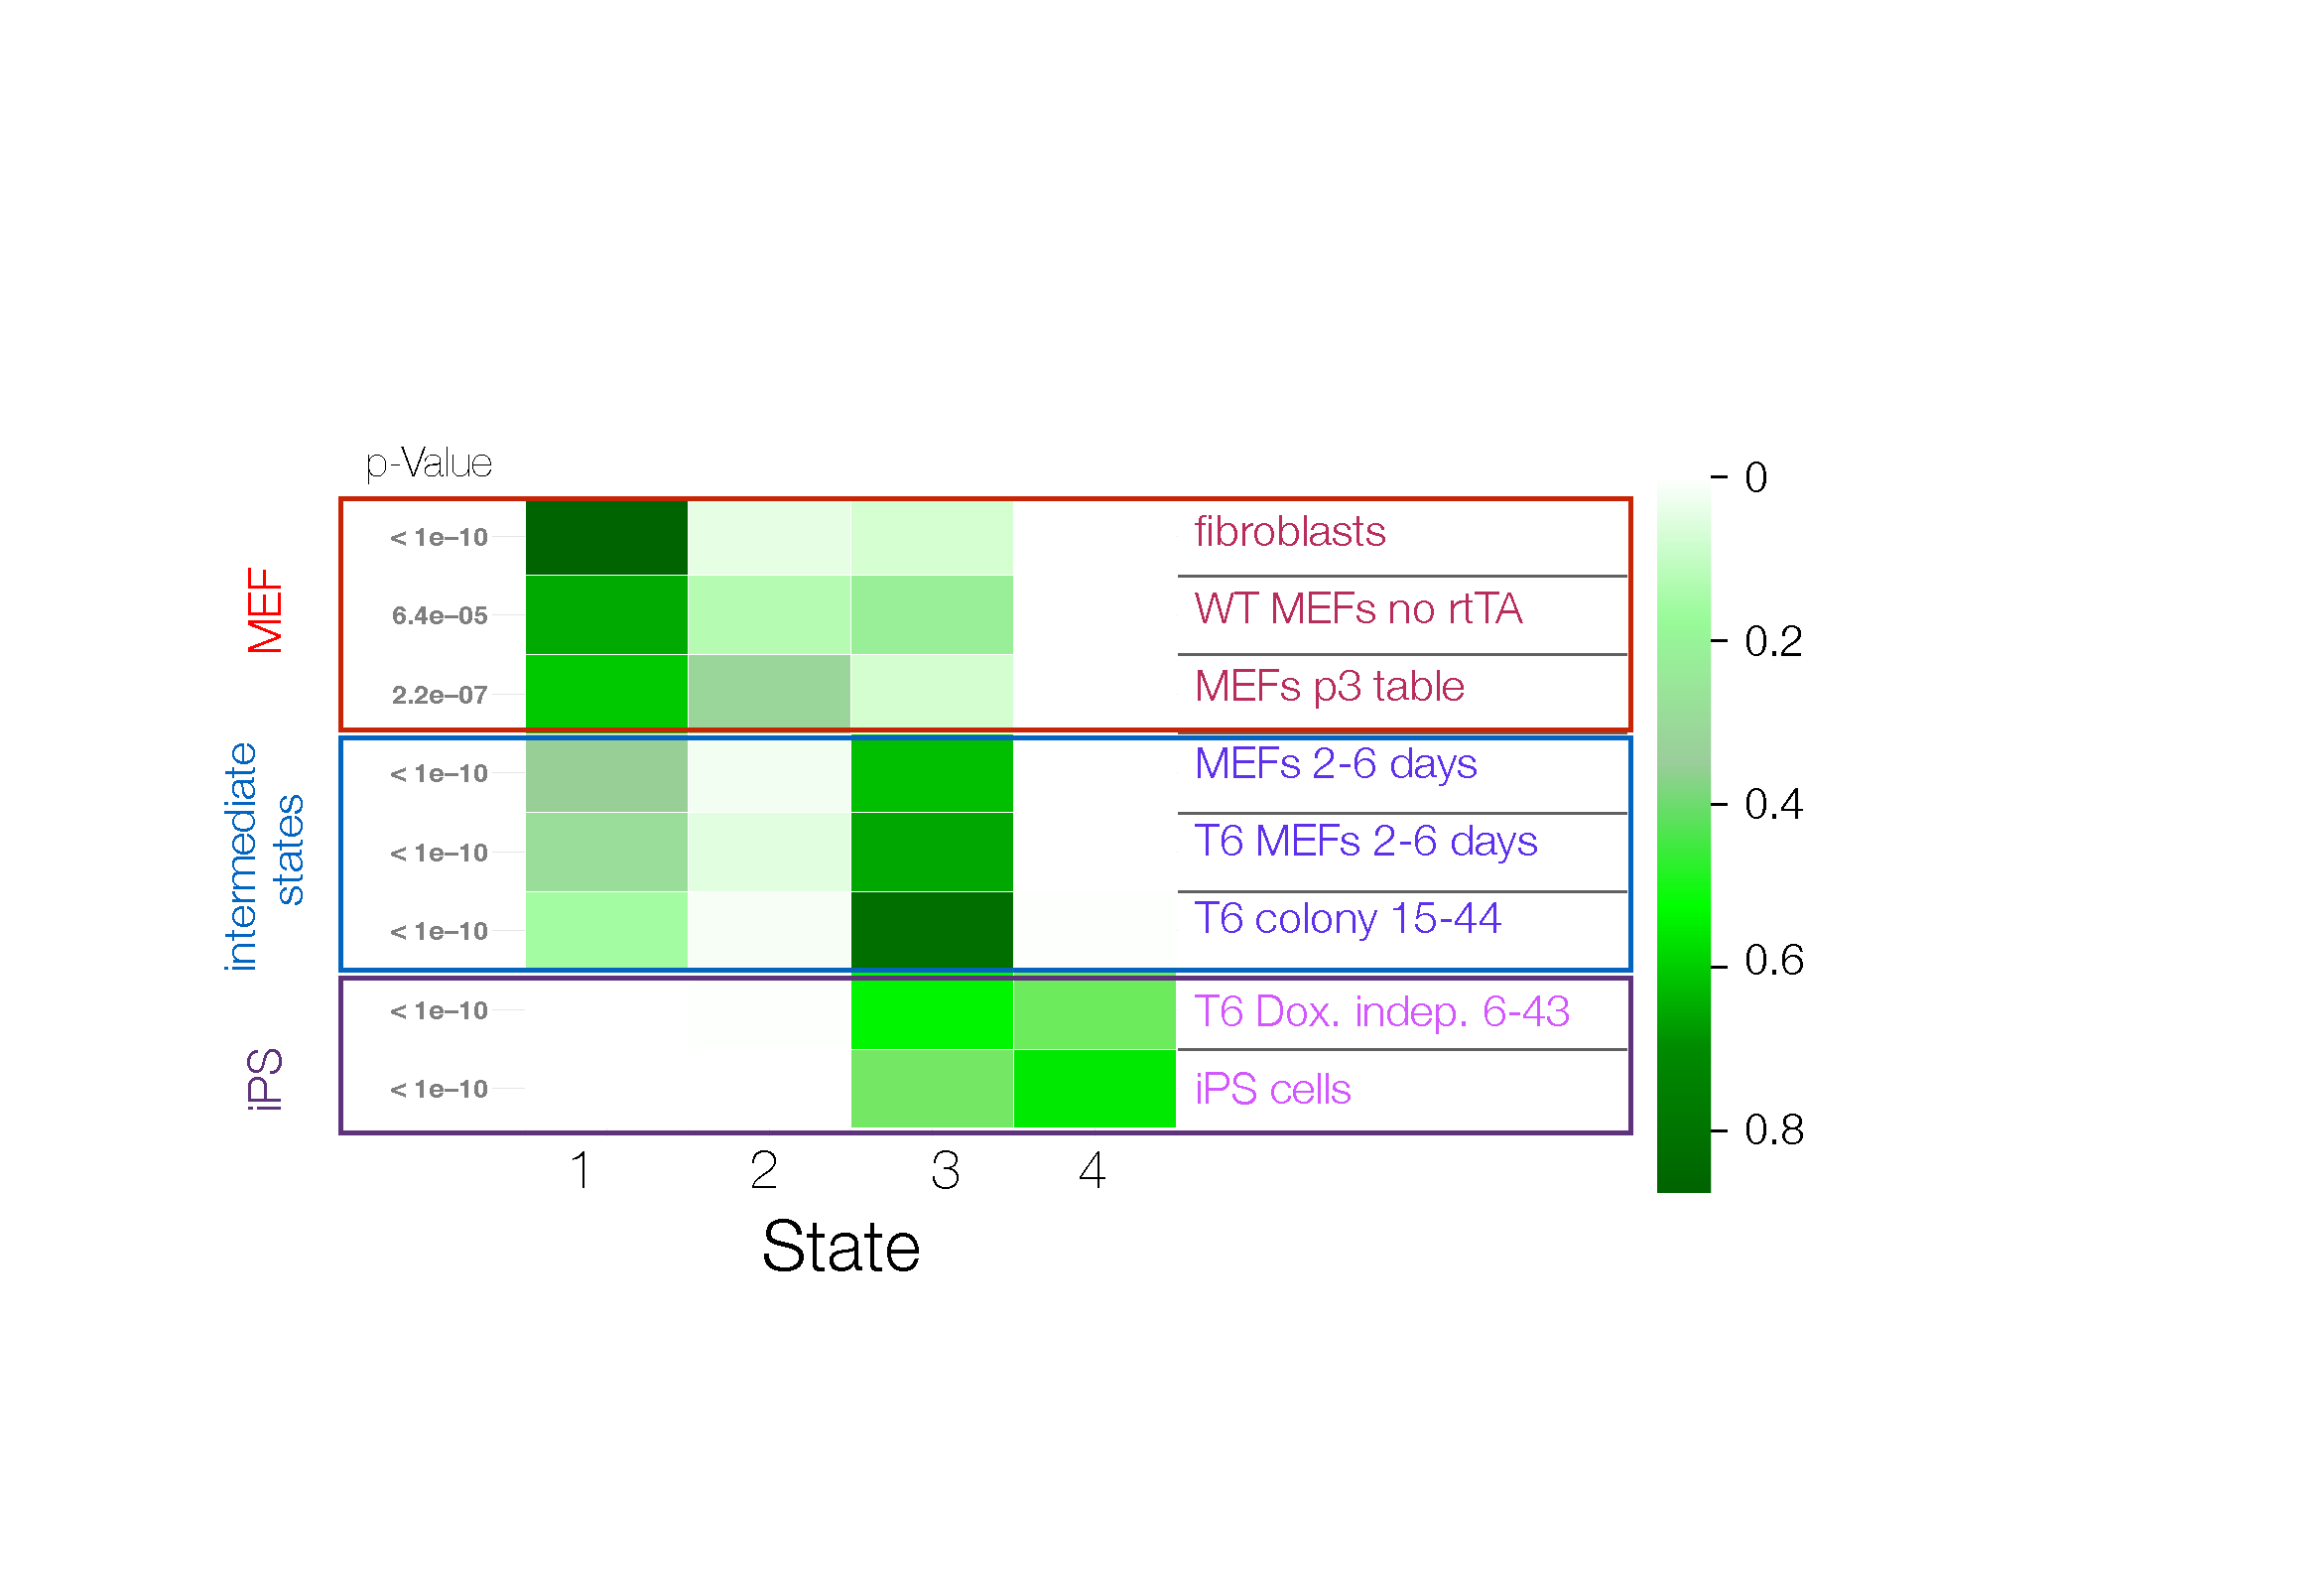
\includegraphics[width=0.9\textwidth]{pics/Heat_single_cells.pdf}
  \caption{Estimated gene expression signatures using STAMM are compared with single-cell measurements, performed by \cite{Buganim:2012hp}. Each single-cell is assigned to a state by finding minimum euclidean distance. The heatmap summarises the fraction of cells from each experimental condition, assigned to specific states. Different conditions show a clear preference for specific states. Predictions from our model are in line with this observation where initial MEF states undergo a transformation via intermediate states to a final reprogrammed state. As an example all MEF populations (top three entries) have a significantly higher fraction of cells in $K=1$. Cells measured between $t=2$ and $t=44$ days have cells that spread across the first and third state, with very few cells occupying the second state. None of these cells are close to the final state. The two measurements which are reprogrammed cells (iPS cells and Dox. indep.) show similarities to $K=3$ and $K=4$, but none of these cells are close to the first two states.
}
  \label{fig:buganim-heat}
\end{figure}

\section{Discussion}
\label{sec:discussion-ips}

We showed how STAMM can be applied to the transformation of differentiated cells from MEF to iPS cells with the help of reprogramming factors. The data used for the first part of the analysis was a population averaged microarray time-course. We outlined the procedure used in \cite{Armond:2013} highlighting differences to the estimation pipeline introduced in Section \ref{cha:stamm}. We present results from fitting STAMM to the data and we find that a four state model best describes stem-cell reprogramming, which has also been corroborated by previous experiments \citep{SamavarchiTehrani:2010cp}. Additionally we showed that data indeed has underlying  structure that can be described by STAMM. To test this we performed estimation for ten samples with randomly permuted time points and compare RSS scores, condition number and Bayesian model selection. We found that RSS and condition number are always lower for the original data than the permuted data. The Bayesian model selection result show a very high concentration at $K=1$ states for the permuted data compared to a high concentration at $K=4$ for the original data. Both results hint that the model is approximating an underlying structure in the data, as fits with permuted data are systematically worse.

We also compared model predictions from STAMM to the single-cell data, obtained in a different secondary MEF experiment measuring $48$ genes for $96$ single-cells \citep{Buganim:2012hp}. We used a standard clustering tool and determined only $3$ states in the data which can either mean that there is not sufficient information available or that intermediate states are characterised by genes not measured in this experiment. If we map single-cell measurements at different time points to gene expression signatures we find that single-cells measured at different times are close to the states predicted by our model at those times. These results are encouraging but for them to be conclusive, as mentioned above, we would need to carry out further experiments.


%%% Local Variables:
%%% TeX-master: "warwickthesis"
%%% End:
